\documentclass[tikz]{standalone}

\usepackage[latin1]{inputenc}
\usepackage{tikz}

\begin{document}
\pagestyle{empty}

\newcommand\rad{0.4}

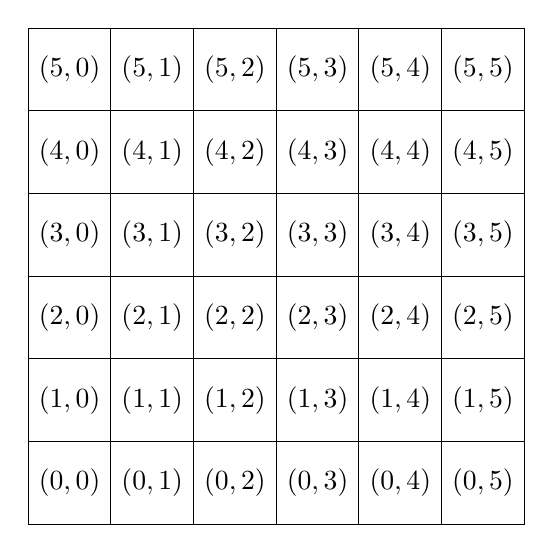
\begin{tikzpicture}[scale=0.7]
    \def\size {5}
    \def\cellscale {1.5}
    \foreach \x in {0,...,\size}
        \foreach \y in {\size,...,0}
        {
            \draw (\cellscale*\x,\cellscale*\y) rectangle +(\cellscale, \cellscale);
            \draw (\cellscale*\x + \cellscale/2,\cellscale*\y + \cellscale/2) node{$(\y,\x)$};
        }
\end{tikzpicture}



\end{document}
